\documentclass{beamer}
\usetheme{Madrid}
\usecolortheme{whale}

% Paquetes necesarios
\usepackage[utf8]{inputenc}
\usepackage[T1]{fontenc}
\usepackage[english]{babel}
\usepackage{amsmath}
\usepackage{amsthm}
\usepackage{tikz}
\usepackage{booktabs}

% Configuración para los logos
\usepackage{tikz}

% Opción 1: Aumentar la altura y profundidad
\setbeamertemplate{footline}{
  \leavevmode%
  \hbox{%
    % Logo izquierdo
    \begin{beamercolorbox}[wd=.3\paperwidth,ht=4.5ex,dp=3ex]{author in head/foot}%
      \hspace*{2ex}
\includegraphics[height=4ex]{Imagenes/Logo Elcano.png}
    \end{beamercolorbox}%
    % Espacio central
    \begin{beamercolorbox}[wd=.4\paperwidth,ht=4.5ex,dp=3ex,center]{title in head/foot}%
      \usebeamerfont{title in head/foot}\insertshortdate{}
    \end{beamercolorbox}%
    % Logo derecho
    \begin{beamercolorbox}[wd=.3\paperwidth,ht=4.5ex,dp=3ex,right]{date in head/foot}%
      
\includegraphics[height=4ex]{Imagenes/logo upo.png}\hspace*{2ex}
    \end{beamercolorbox}}%
  \vskip0pt%
}

% Opción 2: Aún más grande
\setbeamertemplate{footline}{
  \leavevmode%
  \hbox{%
    % Logo izquierdo
    \begin{beamercolorbox}[wd=.3\paperwidth,ht=6ex,dp=4ex]{author in head/foot}%
      \hspace*{2ex}
\includegraphics[height=5ex]{Imagenes/Logo Elcano.png}
    \end{beamercolorbox}%
    % Espacio central
    \begin{beamercolorbox}[wd=.4\paperwidth,ht=6ex,dp=4ex,center]{title in head/foot}%
      \usebeamerfont{title in head/foot}\insertshortdate{}
    \end{beamercolorbox}%
    % Logo derecho
    \begin{beamercolorbox}[wd=.3\paperwidth,ht=6ex,dp=4ex,right]{date in head/foot}%
      
\includegraphics[height=5ex]{Imagenes/logo upo.png}\hspace*{2ex}
    \end{beamercolorbox}}%
  \vskip0pt%
}

\title{Un indicador de seguridad económica para la UE}
\author[Hidalgo, Díaz-Lanchas \& Otero]{
    Manuel Hidalgo-Pérez\inst{1} \and 
    Jorge Díaz-Lanchas\inst{2} \and 
    Miguel Otero\inst{3}
}
\institute[UPO \& RIE]{
    \inst{1} Universidad Pablo de Olavide y Real Instituto Elcano \\
    \inst{2} Universidad Pontificia de Comillas \\
    \inst{3} Real Instituto Elcano
}
\date{\today}

\begin{document}

\begin{frame}
    \titlepage
\end{frame}

\begin{frame}{Índice}
    \tableofcontents
\end{frame}

\section{Motivación y Objetivos}
\begin{frame}
    \centering
    \Huge{Motivación y Objetivos}
\end{frame}


\begin{frame}{Motivación y Objetivos}
    \begin{itemize}
        \item Medir dependencia comercial entre países
        \item Evaluar riesgos de dependencia excesiva
        \item Limitaciones del indicador actual del BCE (CD2)
        \item Necesidad de considerar efectos indirectos
        \item Se complementa con un análisis de cluster que agrupe países por nivel de riesgo geopolítico-económico
    \end{itemize}
\end{frame}

\section{Limitaciones del Indicador Actual}

\begin{frame}
    \centering
    \Huge{Limitaciones de los Indicadores Actuales y propósito de este trabajo}
\end{frame}


\begin{frame}{Indicador CD2 del BCE}
    \begin{itemize}
        \item El BCE utiliza el indicador CD2, entre otros, para medir dependencias comerciales
        \item Definición matemática:
        \[ CD2_{ij} = \frac{M_{ij}}{M_{i} + Y_i} \]
        donde:
        \begin{itemize}
            \item $M_{ij}$: Importaciones del país $i$ desde el país $j$
            \item $M_{i}$: Total de importaciones del país $i$
            \item $Y_i$: Producción doméstica del país $i$
        \end{itemize}
    \end{itemize}
\end{frame}

\begin{frame}{Limitaciones del CD2}
    \begin{block}{Principales problemas}
        \begin{enumerate}
            \item Solo captura dependencias directas
            \item Ignora efectos de red en comercio internacional
            \item No considera "hubs" comerciales intermedios
        \end{enumerate}
    \end{block}
    
    \begin{block}{Ejemplo}
        Si España importa de Alemania, y Alemania depende de China:
        \begin{itemize}
            \item CD2 no captura la dependencia indirecta España-China
            \item Subestima la vulnerabilidad real
            \item Ignora las cadenas de valor globales
        \end{itemize}
    \end{block}
\end{frame}

\begin{frame}{Propósito de este nuevo indicador}
    \begin{block}{Resolver estos principales problemas}
        \begin{enumerate}
            \item Captura dependencias directas e indirectas
            \item Tener en cuenta los efectos de red en comercio internacional
            \item Tener en cuenta los "hubs" comerciales intermedios
        \end{enumerate}
    \end{block}
\end{frame}

\section{Metodología}
\begin{frame}
    \centering
    \Huge{Metodología}
\end{frame}

\begin{frame}{Dependencia Directa vs Indirecta}
    \begin{itemize}
        \item Dependencia directa: importaciones directas del país E
        \item Dependencia indirecta: a través de países intermediarios
        \item Efecto "hub" en el comercio internacional
        \item Importancia de las cadenas comerciales globales
    \end{itemize}
\end{frame}

\begin{frame}{Estructura de Dependencias}
    \centering
    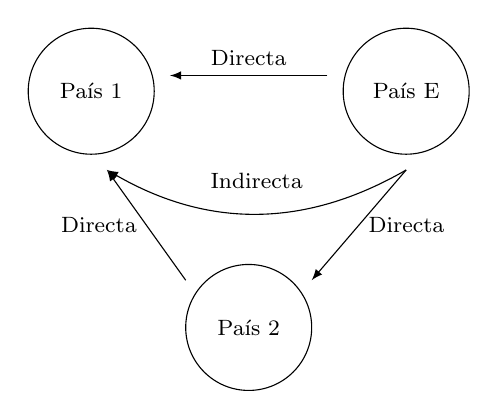
\begin{tikzpicture}[font=\footnotesize]
        % Círculos 1 y E (mantienen su posición)
        \draw (0,0) circle (0.8cm) node {País 1};
        \draw (4,0) circle (0.8cm) node {País E};
        
        % Círculo 2 (más abajo)
        \draw (2,-3) circle (0.8cm) node {País 2};  % Cambiado de -2 a -3
    
        % Flecha directa entre E y 1 (mantiene su posición)
        \draw [-latex] (3,0.2) -- (1,0.2) node [midway,above] {Directa};
        
        % Flechas hacia/desde 2 (ajustadas a la nueva posición)
        \draw [-latex] (4,-1) -- (2.8,-2.4) node [midway,right] {Directa};
        \draw [-latex] (1.2,-2.4) -- (0.2,-1) node [midway,left] {Directa};

        % Flecha curva indirecta (ajustada)
        \draw [-latex, bend left] (4,-1) to node[above=0.2cm] {Indirecta} (0.2,-1);
    \end{tikzpicture}
\end{frame}


\begin{frame}{Formulación Matemática Básica (para tres países más el país con el que medir la dependencia--> E)}
    \begin{itemize}
        \item Dependencia directa del país 1 respecto a E:
        \[ a_{E1} = \frac{x_{E1}}{x_{E1}+x_{21}+x_{31}+x_{11}} \]
        donde:
        \begin{itemize}
            \item $x_{E1}$: importaciones del país 1 desde E
            \item $x_{i1}$: importaciones del país 1 desde país i
            \item Denominador: disponibilidades totales del país 1
        \end{itemize}
        \end{itemize}
\end{frame}
\begin{frame}{Formulación Matemática Básica (para tres países más el país con el que medir la dependencia--> E)}
    \begin{itemize}
    \item Matriz de comercio bilateral:
        \[ X =
        \begin{bmatrix}
        x_{11} & x_{12} & x_{13} & x_{1E} \\
        x_{21} & x_{22} & x_{23} & x_{2E} \\
        x_{31} & x_{32} & x_{33} & x_{3E} \\
        x_{E1} & x_{E2} & x_{E3} & x_{EE}
        \end{bmatrix} \]
        \begin{itemize}
            \item $x_{ij}$: flujo comercial desde j hacia i
            \item Diagonal: producción doméstica
        \end{itemize}
    \end{itemize}
\end{frame}

\begin{frame}{Matriz de Dependencia (coeficientes)}

    Definimos la matriz $A$ de dependencia como :
    \begin{align*}
    A=
    \begin{bmatrix}
    a_{11} & a_{12} & a_{13} & a_{1E} \\
    a_{21} & a_{22} & a_{23} & a_{2E} \\
    a_{31} & a_{32} & a_{33} & a_{3E} \\
    a_{E1} & a_{E2} & a_{E3} & a_{EE}
    \end{bmatrix}
    \end{align*}
    donde las $a_{ij}$ se obtienen del mismo modo que el CD2 y cuya representación más general sería:
    \begin{align*}
        a_{ij} = \frac{x_{ij}}{\sum_{j} x_{ij}}
    \end{align*}
    \begin{align*}
        i,j\in{1,2,3,E}
    \end{align*}
\end{frame}

\begin{frame}{Matriz de Dependencia de países intermedios}
    \begin{block}{Matriz de dependencia intermedia. Eliminando E}
        \[ A_{\Omega} \subseteq A', \quad \Omega = \{1, 2, 3\} \]
    \end{block}
\end{frame}

\begin{frame}{Estructura de Dependencias}
    \centering
    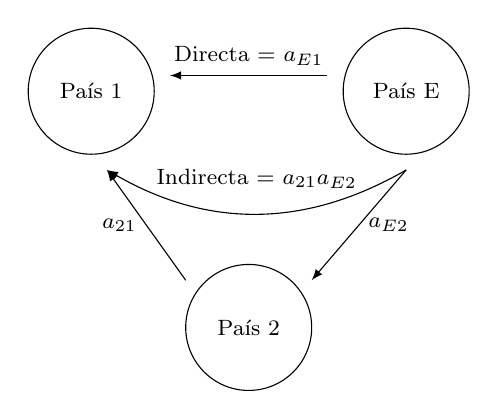
\begin{tikzpicture}[font=\footnotesize]
        % Círculos 1 y E (mantienen su posición)
        \draw (0,0) circle (0.8cm) node {País 1};
        \draw (4,0) circle (0.8cm) node {País E};
        
        % Círculo 2 (más abajo)
        \draw (2,-3) circle (0.8cm) node {País 2};
    
        % Flecha directa entre E y 1
        \draw [-latex] (3,0.2) -- (1,0.2) node [midway,above] {Directa = $a_{E1}$};
        
        % Flechas hacia/desde 2 con coeficientes
        \draw [-latex] (4,-1) -- (2.8,-2.4) node [midway,right] {$a_{E2}$};
        \draw [-latex] (1.2,-2.4) -- (0.2,-1) node [midway,left] {$a_{21}$};
        
        % Flecha curva indirecta
        \draw [-latex, bend left] (4,-1) to node[above=0.2cm] {Indirecta = $a_{21}a_{E2}$} (0.2,-1);
    \end{tikzpicture}
    
    \vspace{0.5cm} % Espacio entre el diagrama y el texto
    \small % Tamaño de texto más pequeño para el texto explicativo
    $\delta = a_{E1} + a_{21} \cdot a_{E2}$
\end{frame}

\begin{frame}{Dependencias Indirectas - Ejemplo}
    Consideremos la dependencia de España (1) de China (E) vía Alemania (2):
    \begin{itemize}
        \item España importa de Alemania: $a_{21}$ = 30\%
        \item Alemania depende de China: $a_{E2}$ = 40\%
        \item Dependencia indirecta: $0.3 \times 0.4 = 12\%$
        \item Esta es solo una de las múltiples rutas posibles
    \end{itemize}
\end{frame}

\begin{frame}{Dependencias Indirectas}
    \begin{block}{Nivel 2 de dependencia (con dos países intermedios)}
        \[ \delta_1^2 = a_{21} \cdot a_{E2} + a_{31} \cdot a_{E3} \]
        \begin{itemize}
            \item $a_{21} \cdot a_{E2}$: dependencia vía país 2
            \item $a_{31} \cdot a_{E3}$: dependencia vía país 3
            \item Suma de todas las rutas indirectas de longitud 2
        \end{itemize}
    \end{block}
\end{frame}

\begin{frame}{Dependencia Total}    
    \begin{block}{Dependencia total}
        \[ \delta = a_E\left[I-A_{\Omega}\right]^{-1} \]
        \begin{itemize}
            \item Suma infinita de todos los niveles de dependencia
            \item $[I-A_{\Omega}]^{-1}$: matriz de Leontief inversa
            \item Captura todas las conexiones posibles
        \end{itemize}
    \end{block}
\end{frame}



\begin{frame}{Caso de Dos Países Externos}
    \begin{block}{Extensión del modelo base}
        Para países $E_1$ (p.ej., China) y $E_2$ (p.ej., Rusia):
        \begin{itemize}
            \item Matrices separadas:
            \begin{itemize}
                \item $A_1$: matriz de dependencias respecto a $E_1$
                \item $A_2$: matriz de dependencias respecto a $E_2$
            \end{itemize}
            \item Dependencias directas: 
            \begin{itemize}
                \item $\delta^1_1 = a_{E_1}$: vector de dependencias directas de $E_1$
                \item $\delta^1_2 = a_{E_2}$: vector de dependencias directas de $E_2$
            \end{itemize}
        \end{itemize}
    \end{block}
    
    \begin{block}{Dependencias totales}
        \[ \delta_1 = a_{E_1} [I - A_{\Omega_1}]^{-1} \]
        \[ \delta_2 = a_{E_2} [I - A_{\Omega_2}]^{-1} \]
        Captura todas las rutas posibles a través de cualquier país intermediario
    \end{block}
\end{frame}
\section{Concentración de la Dependencia}

\begin{frame}{Se debe acompañar de un análsis de concentración}
    \begin{block}{¿Por qué?}
        La dependencia alta no es el único riesgo:
        \begin{itemize}
            \item País A: 40\% dependencia repartida entre 10 países
            \item País B: 40\% dependencia concentrada en 2 países
            \item \alert{Mismo nivel de dependencia, pero diferente riesgo al estar más concentrada respecto a B}
        \end{itemize}
    \end{block}
\end{frame}

\begin{frame}
    \begin{block}{Solución: Índice de Herfindahl}
        \[ H_j = \sum_{i=1}^{n} s_{ij}^2 \]
        Nos permite:
        \begin{itemize}
            \item Medir concentración de dependencias
            \item Identificar vulnerabilidades adicionales
            \item Evaluar diversificación de proveedores
        \end{itemize}
    \end{block}
\end{frame}

\begin{frame}
    \begin{example}
        España en "Processing of nuclear fuel":
        \begin{itemize}
            \item Alta dependencia (2.23)
            \item Distribuida entre 5 países principales
            \item Menor riesgo que sectores con dependencia similar pero más concentrada
        \end{itemize}
    \end{example}
\end{frame}

\section{Resultados para España}

\begin{frame}{Base de Datos y Alcance}
    \begin{itemize}
        \item Utilizamos la International Trade and Production Database (ITP)
        \item Análisis centrado en el año 2019
        \item Cobertura:
            \begin{itemize}
                \item Datos de comercio bilateral
                \item 170 productos
                \item 237 países
                \item Más de 2,5 millones de datos por año
                \item Incluye producción doméstica
                \item Todas las industrias manufactureras 
            \end{itemize}
        \item Ventajas:
            \begin{itemize}
                \item Desagregación por industrias
                \item Cobertura global
                \item Homogeneidad en la medición
                \item El método puede implementarse para otras bases de datos
            \end{itemize}
    \end{itemize}
\end{frame}

\begin{frame}{Proceso de Implementación}
    \begin{block}{Etapas del análisis}
        \begin{enumerate}
            \item \textbf{Preparación de datos}
                \begin{itemize}
                    \item Organización por industrias
                    \item Identificación de países y sus relaciones
                \end{itemize}
            \item \textbf{Análisis de dependencias directas}
                \begin{itemize}
                    \item Creación de matrices de comercio bilateral
                    \item Cálculo de proporciones de dependencia
                \end{itemize}
            \item \textbf{Análisis de dependencias indirectas}
                \begin{itemize}
                    \item Identificación de rutas comerciales intermedias
                    \item Cálculo de efectos acumulados
                \end{itemize}
        \end{enumerate}
    \end{block}
\end{frame}

\begin{frame}{Ventajas del Nuevo Enfoque}
    \begin{columns}[t]
        \begin{column}{0.5\textwidth}
            \textbf{Aspectos Técnicos}
            \begin{itemize}
                \item Automatización completa
                \item Procesamiento eficiente
                \item Actualización sencilla
            \end{itemize}
        \end{column}
        \begin{column}{0.5\textwidth}
            \textbf{Beneficios Analíticos}
            \begin{itemize}
                \item Visión completa de dependencias
                \item Identificación de vulnerabilidades ocultas
                \item Análisis por sectores
            \end{itemize}
        \end{column}
    \end{columns}
\end{frame}

\begin{frame}{Del Dato al Conocimiento}
    \begin{block}{Proceso de transformación}
        \begin{enumerate}
            \item \textbf{Entrada}: Datos comerciales brutos
            \item \textbf{Procesamiento}: 
                \begin{itemize}
                    \item Matrices de relaciones comerciales
                    \item Cálculos de dependencias
                \end{itemize}
            \item \textbf{Salida}: 
                \begin{itemize}
                    \item Índices de dependencia por sector
                    \item Mapas de vulnerabilidad
                    \item Recomendaciones de política
                \end{itemize}
        \end{enumerate}
    \end{block}
\end{frame}

\begin{frame}{Principales Dependencias}
    \centering
    \scriptsize
    Sectores más dependientes:
    \vspace{0.3cm} % Espacio entre el título y la tabla para mejorar la estética
    \begin{tabular}{|p{6.5cm}|c|c|}
        \hline
        \textbf{Sector} & \textbf{Dependencia} & \textbf{HFD} \\
        \hline
        Manufacturing services on physical inputs owned by others & 2.85 & 1.17 \\
        Animal feed ingredients and pet foods                     & 2.29 & 0.53 \\
        Processing of nuclear fuel                                & 2.24 & 0.88 \\
        Electricity distribution \& control apparatus             & 2.21 & 0.53 \\
        Live Cattle                                               & 2.17 & 0.65 \\
        Forestry                                                  & 2.16 & 0.21 \\
        Other meats, livestock products, and live animals         & 2.14 & 0.51 \\
        Other publishing                                          & 2.13 & 0.72 \\
        Jewellery and related articles                            & 2.11 & 0.42 \\
        Fishing                                                   & 2.08 & 0.35 \\
        \hline
    \end{tabular}
\end{frame}



\begin{frame}{Ejemplo: Nuclear Fuel}
    \centering
    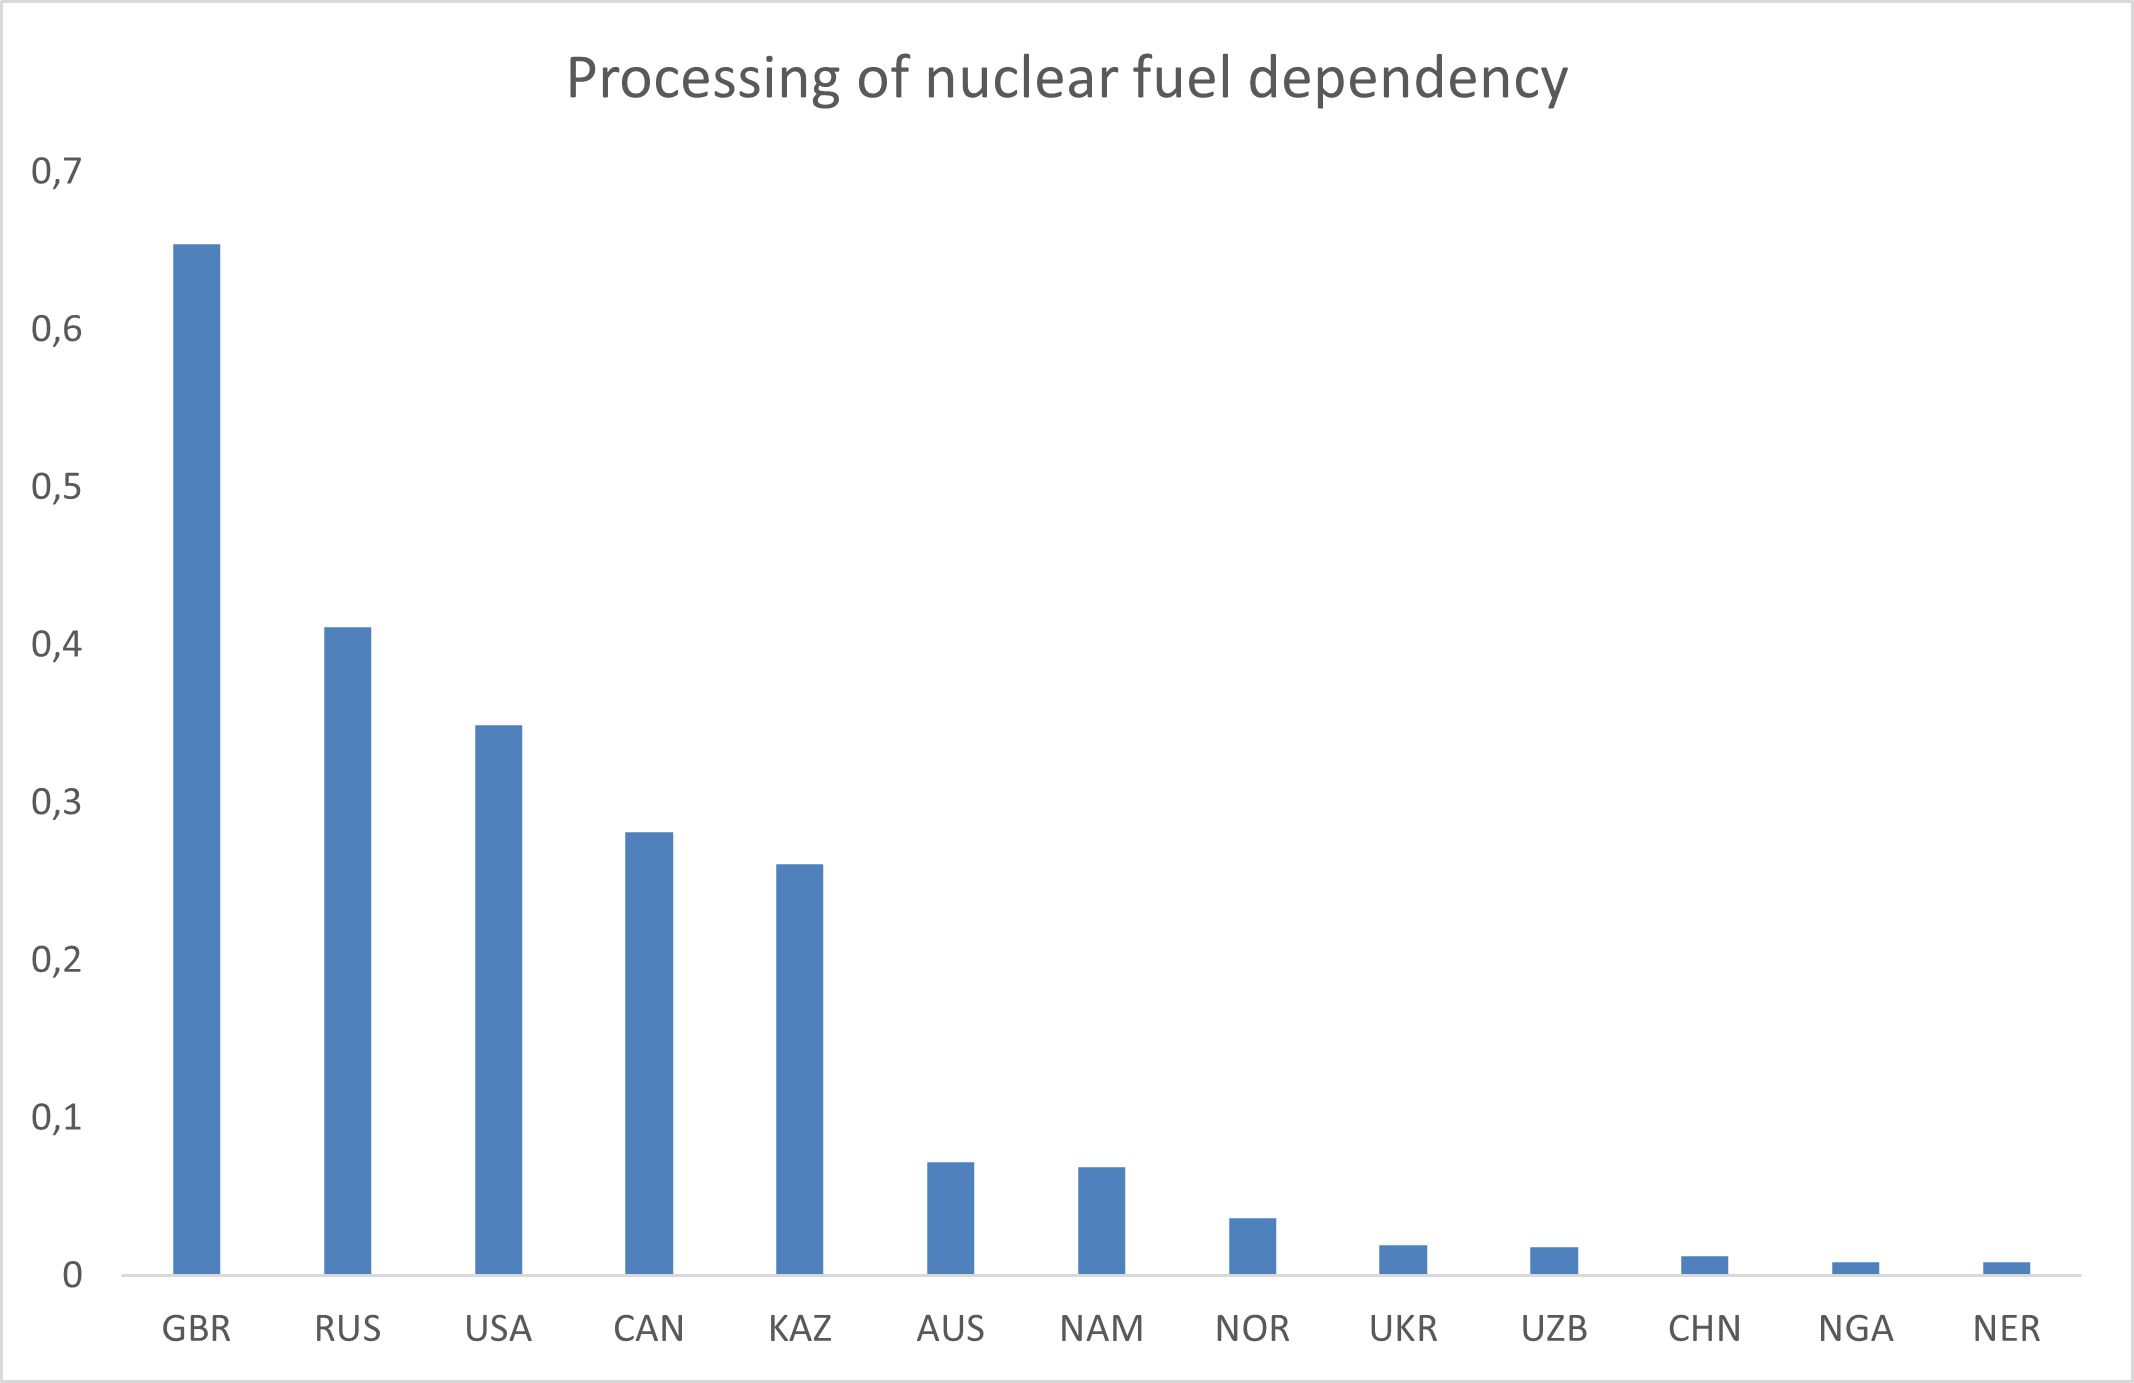
\includegraphics[width=0.8\linewidth]{../Imagenes/Nuclear fig.png}
    
\end{frame}



%----------------------------------------------------------------

\section{Análisis de Riesgo Geopolítico}
\begin{frame}
    \centering
    \Huge{Análisis de Riesgo Geopolítico}
\end{frame}
\section{Análisis de Riesgo Geopolítico}


\begin{frame}{¿Por qué necesitamos agrupar países por riesgo?}
    \begin{block}{Limitaciones del análisis puramente económico}
        \begin{itemize}
            \item La dependencia comercial no captura todo el riesgo
            \item Factores geopolíticos afectan a la seguridad económica
            \item Necesidad de una visión más completa del riesgo
        \end{itemize}
    \end{block}
    
    \begin{block}{Objetivos}
        \begin{itemize}
            \item Capturar tensiones geopolíticas actuales
            \item Identificar alineaciones políticas
            \item Considerar factores históricos y culturales
        \end{itemize}
    \end{block}
\end{frame}

\begin{frame}{Dimensiones del Riesgo}
    \begin{columns}[t]
        \begin{column}{0.33\textwidth}
            \textbf{Económica}
            \begin{itemize}
                \item Dependencias comerciales
                \item Acuerdos económicos
                \item Sanciones financieras
            \end{itemize}
        \end{column}
        \begin{column}{0.33\textwidth}
            \textbf{Geopolítica}
            \begin{itemize}
                \item Alianzas políticas
                \item Conflictos actuales
                \item Posiciones diplomáticas
            \end{itemize}
        \end{column}
        \begin{column}{0.33\textwidth}
            \textbf{Cultural}
            \begin{itemize}
                \item Historia compartida
                \item Proximidad cultural
                \item Sistemas legales
            \end{itemize}
        \end{column}
    \end{columns}
\end{frame}

\begin{frame}{Capturando el Contexto Actual}
    \begin{block}{Elementos clave considerados}
        \begin{itemize}
            \item \textbf{Crisis de Ucrania}
                \begin{itemize}
                    \item Posiciones en votaciones de la ONU
                    \item Participación en iniciativas de paz (Suiza)
                    \item Aplicación de sanciones
                \end{itemize}
            \item \textbf{Tensiones globales}
                \begin{itemize}
                    \item Relaciones con China
                    \item Alineación con bloques principales
                    \item Restricciones comerciales
                \end{itemize}
        \end{itemize}
    \end{block}
\end{frame}

\begin{frame}{Factores Históricos y Culturales}
    \begin{itemize}
        \item \textbf{Relaciones históricas}
            \begin{itemize}
                \item Vínculos coloniales pasados
                \item Influencia en relaciones actuales
            \end{itemize}
        \item \textbf{Proximidad cultural}
            \begin{itemize}
                \item Similitud lingüística
                \item Sistemas legales comunes
            \end{itemize}
        \item \textbf{Geografía}
            \begin{itemize}
                \item Pertenencia a continentes
                \item Proximidad regional
            \end{itemize}
    \end{itemize}
\end{frame}

\begin{frame}{Alineaciones Políticas Globales}
    \begin{block}{Principales bloques considerados}
        \begin{itemize}
            \item \textbf{Occidente}
                \begin{itemize}
                    \item Alineación con EE.UU.
                    \item Relación con la UE
                \end{itemize}
            \item \textbf{Este}
                \begin{itemize}
                    \item Relación con China
                    \item Posición respecto a Rusia
                \end{itemize}
        \end{itemize}
    \end{block}
    
    \begin{alertblock}{¿Por qué es importante?}
        Las alineaciones políticas pueden anticipar:
        \begin{itemize}
            \item Futuros conflictos comerciales
            \item Riesgos en cadenas de suministro
            \item Potenciales sanciones
        \end{itemize}
    \end{alertblock}
\end{frame}

\begin{frame}{Sanciones y Restricciones}
    \begin{itemize}
        \item \textbf{Tipos de medidas analizadas}
            \begin{itemize}
                \item Restricciones comerciales
                \item Sanciones financieras
                \item Limitaciones de viaje
                \item Embargos de armas
            \end{itemize}
        \item \textbf{Importancia}
            \begin{itemize}
                \item Indicadores de tensión política
                \item Impacto en relaciones económicas
                \item Señales de alerta temprana
            \end{itemize}
    \end{itemize}
\end{frame}

\begin{frame}{Construcción del Índice Final}
    \begin{block}{Tres dimensiones integradas}
        \begin{enumerate}
            \item \textbf{Riesgo económico}
                \begin{itemize}
                    \item Basado en dependencias comerciales
                    \item Concentración de proveedores
                \end{itemize}
            \item \textbf{Riesgo geopolítico}
                \begin{itemize}
                    \item Tensiones internacionales
                    \item Alineaciones políticas
                \end{itemize}
            \item \textbf{Riesgo cultural}
                \begin{itemize}
                    \item Distancia cultural e histórica
                    \item Barreras potenciales
                \end{itemize}
        \end{enumerate}
    \end{block}
\end{frame}

\subsection{Reducción de Dimensionalidad}

\begin{frame}
    \centering
    \Huge{Reducción de Dimensionalidad: \\
    Simplificando la Complejidad}
\end{frame}

\begin{frame}{¿Por qué reducir dimensiones?}
    \begin{block}{El reto de la complejidad}
        \begin{itemize}
            \item Múltiples variables por cada dimensión
            \item Información redundante o correlacionada
            \item Dificultad para visualizar y analizar
        \end{itemize}
    \end{block}
    
    \begin{alertblock}{Objetivo}
        Convertir información compleja en índices manejables sin perder información relevante
    \end{alertblock}
\end{frame}

\begin{frame}{Tres Dimensiones Principales}
    \begin{columns}[t]
        \begin{column}{0.32\textwidth}
            \textbf{Geopolítica}
            \centering
            \begin{itemize}
                \item Alineaciones
                \item Tensiones
                \item Sanciones
            \end{itemize}
        \end{column}
        \begin{column}{0.32\textwidth}
            \textbf{Cultural}
            \centering
            \begin{itemize}
                \item Historia
                \item Lengua
                \item Sistema legal
            \end{itemize}
        \end{column}
        \begin{column}{0.32\textwidth}
            \textbf{Comercial}
            \centering
            \begin{itemize}
                \item Acuerdos
                \item Barreras
                \item Cooperación
            \end{itemize}
        \end{column}
    \end{columns}
\end{frame}

\begin{frame}{Dimensión Geopolítica}
    \begin{block}{De la complejidad a la simplicidad}
        \textbf{Variables de entrada:}
        \begin{itemize}
            \item Alineación con bloques de poder
            \item Posiciones en conflictos
            \item Sanciones internacionales
        \end{itemize}
        
        \textbf{Resultado:}
        \begin{itemize}
            \item Un único índice de distancia geopolítica
            \item Escala normalizada de 0 a 1
            \item Fácil interpretación
        \end{itemize}
    \end{block}
\end{frame}

\begin{frame}{Dimensión Cultural}
    \begin{block}{Capturando similitudes y diferencias}
        \textbf{Variables de entrada:}
        \begin{itemize}
            \item Historia colonial compartida
            \item Proximidad lingüística
            \item Sistemas legales comunes
        \end{itemize}
        
        \textbf{Resultado:}
        \begin{itemize}
            \item Índice único de distancia cultural
            \item Considera factores mixtos
            \item Comparable entre países
        \end{itemize}
    \end{block}
\end{frame}

\begin{frame}{Dimensión Comercial}
    \begin{block}{Evaluando vínculos comerciales}
        \textbf{Variables de entrada:}
        \begin{itemize}
            \item Acuerdos comerciales existentes
            \item Barreras comerciales
            \item Cooperación económica
        \end{itemize}
        
        \textbf{Resultado:}
        \begin{itemize}
            \item Índice de similitud comercial
            \item Refleja cercanía económica
            \item Facilita comparaciones
        \end{itemize}
    \end{block}
\end{frame}

\begin{frame}{Resultado Final}
    \begin{center}
        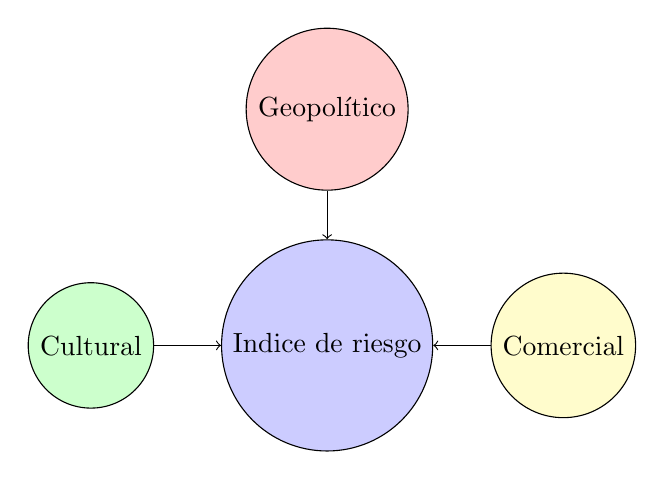
\begin{tikzpicture}
        % Círculo central
            \node[circle,draw,fill=blue!20] (center) {Indice de riesgo};
            % Círculos externos con coordenadas específicas
            \node[circle,draw,fill=red!20] (geo) at (0, 3) {Geopolítico};
            \node[circle,draw,fill=green!20] (cult) at (-3, 0) {Cultural};
            \node[circle,draw,fill=yellow!20] (trade) at (3, 0) {Comercial};
            
            % Conectores
            \draw[->] (geo) -- (center);
            \draw[->] (cult) -- (center);
            \draw[->] (trade) -- (center);
        \end{tikzpicture}
    \end{center}
    
    \begin{itemize}
        \item Tres índices complementarios
        \item Visión completa del riesgo
        \item Base para decisiones informadas
    \end{itemize}
\end{frame}


\begin{frame}
    \begin{figure*} % Utilizamos figure* en lugar de figure
        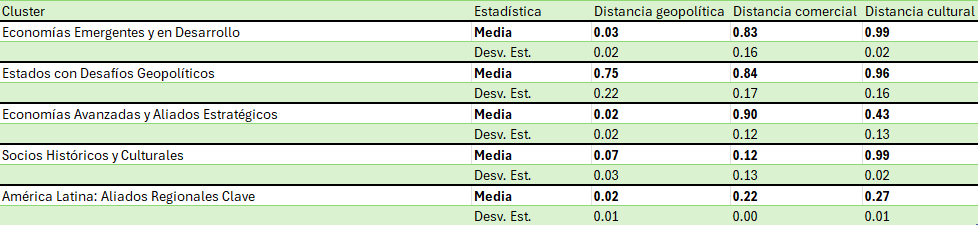
\includegraphics[width=1\linewidth]{Imagenes/tabla clusters.png}
        \label{fig:fig1}
    \end{figure*}
\end{frame}


\begin{frame}
    \begin{figure*} % Utilizamos figure* en lugar de figure
        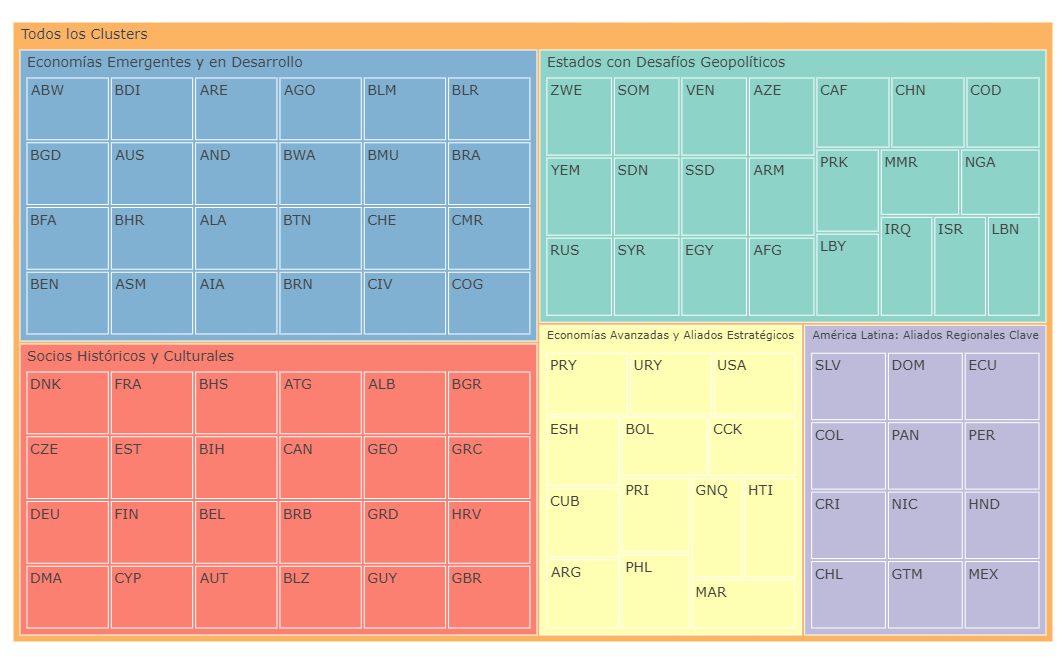
\includegraphics[width=1\linewidth]{Imagenes/geopolitica.png}
        \label{fig:fig1}
    \end{figure*}
\end{frame}

\begin{frame}
    \centering
    \Huge{Muchas gracias}
\end{frame}
\end{document}